%!TEX root = ./../thesis.tex

\chapter{Consistency Management}
\label{c:consistency_mgmt}
Consistency management in the context of distributed machine learning describes the process of ensuring an algorithm is parallelized most efficiently without loosing its correctness.
Iterative-convergent algorithms are mostly sequential in nature and parallelization is commonly achieved by exploiting their inherent stochastic properties.
Staying with the example of the previous section, as shown in Figure \ref{fig:ica_control_flow}, the unit $\Omega_2$ of training step (C) is parallelized with a dop of $k = 2$ by partitioning the input data $D$ and replicating the model $w$ across all parallel units of $\Omega_2$.
Ensuring proper consistency management affects two domains of the algorithm execution process.
First, as discussed in Section \ref{ss:synchronization} the control-flow must be synchronized properly according to the transformation applied during the execution of a unit and its replicas.
In the example, the loop in (B) and its containing units $\Omega_{2i}$ are defined to be SSP in order to increase the data throughput on the input data $D$ and in the end achieve a better overall performance.
Unfortunately, increasing the data throughput alone does not necessarily lead to a better overall performance as each unit $\Omega_{2j}$ now works independently on a replica $w_j$ of the model without sharing the local progress.
As discussed in Section \ref{ss:consistency} this staleness of state has a negative effect on the algorithm throughput and can be mitigated by continuously exchanging the updates applied to a state, in this case $w$, between all units $\Omega_{2j}$.
Exchanging updates on the other hand has a negative effect on the data throughput as more computation time must be spent on network management.
Adaptive consistency management therefore is responsible for controlling the best trade-off between communication and computation, given the requirements for synchronization and consistency at each step of the algorithm.

In order to achieve the greatest flexibility and fine grained control over the consistency during algorithm execution, the consistency management is part of the unit itself.
Figure \ref{fig:unit_internal_flow} depicts the unit internal control flow responsible for executing the actual computation followed by a number of steps related to consistency management.
\begin{figure}[ht]
\centering
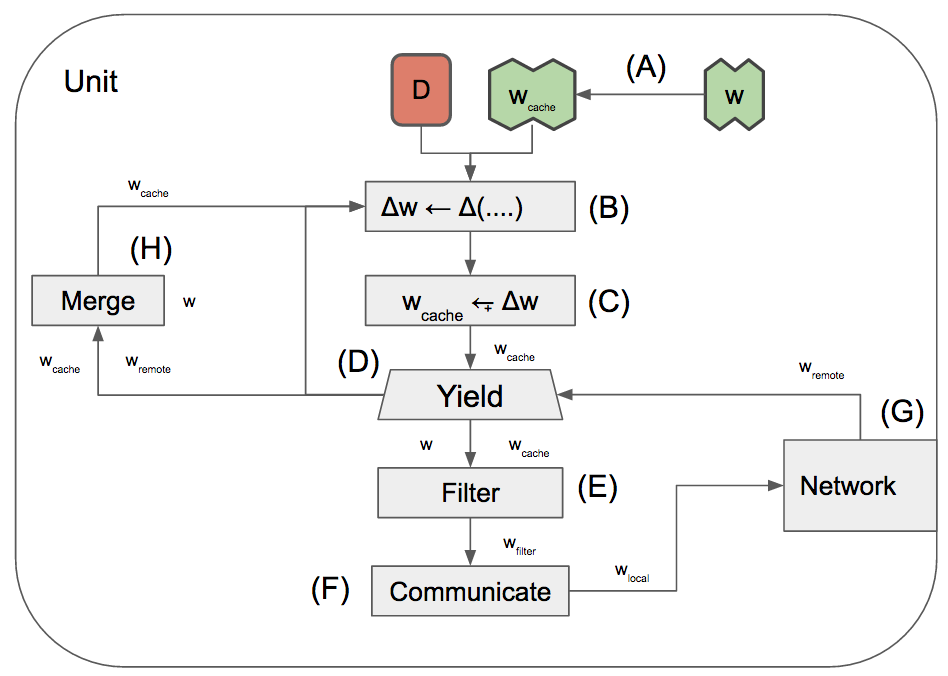
\includegraphics[width=0.9\textwidth]{img/unit_internal_flow.png}
\caption{Unit internal Control-flow}
\label{fig:unit_internal_flow}
\end{figure}
When a unit is executed, the first step (A) is to decide whether it is necessary to cache the updates applied to the output state.
This is necessary because many algorithms require a delta to be communicated instead of the actual value.
In the example, $w$ is cached in $w_{cache}$ at the beginning of the unit execution so $\Delta w = w_{cache} - w$ can be computed if necessary when communicate $\Delta w$ to the corresponding units $\Omega_{ij}$.

- resolving conflicting updates, e.g. when accessing remote state
- deciding when to communicate and what to communicate
- filtering, prioritizing, communicating, merging



	